\section{Synteza dźwięku fletu}

W literaturze można znaleźć wiele różnych metod syntezy dźwięku instrumentów dętych drewnianych. Ich modele są przedstawione zazwyczaj za pomocą różniczkowych równań fizycznych lub w postaci falowodów cyfrowych. 
%klarnet: https://www.researchgate.net/publication/4333455_Representation_of_solo_clarinet_music_by_physical_modeling_synthesis
%gestures: https://www.researchgate.net/publication/5323798_Gesture_synthesis_basic_control_of_a_flute_physical_model
%slide-flute perry cook: https://quod.lib.umich.edu/cache//b/b/p/bbp2372.1992.072/bbp2372.1992.072.pdf#page=1;zoom=75
Przykładem takiej pracy naukowej jest artykuł na temat modelu fizycznego klarnetu, w którym autorzy opisują równaniami różniczkowymi interakcje poszczególnych elementów instrumentu dętego drewnianego \cite{flute_klarnet}. Inna praca naukowa porusza temat sterowania modelem fletu, w którym autorzy skupili się na opisaniu zależności fizycznych związanych głównie z grą flecisty \cite{flute_flecista}. Elementy jakie były brane pod uwagę to ciśnienie w jamie ustnej instumentalisty, odległości warg od ustnika fletu oraz szerokości otwarcia ust grającego. Kolejnym przykładem artykułu opisującego model instrumentu dętego drewnianego jest praca P. Cooka przedstawiająca falowody cyfrowe fletu suwakowego (ang. slide flute) oraz klarnetu \cite{flute_cook}.

W niniejszym podrozdziale przedstawiono dwa podejścia do implementacji syntezy dźwięku drewnianego instrumentu dętego:
\begin{itemize}
	\setlength\itemsep{-3pt}
	\item za pomocą falowodu cyfrowego,
	\item za pomocą zidentyfikowanego modelu ARMA.
\end{itemize}
Na końcu tego podrozdziału przedstawiono porównanie wyników uzyskanych za pomocą obu tych rozwiązań, na podstawie wygenerowanych dźwięków.

\subsection{Synteza falowodowa instrumentów dętych}
%https://ccrma.stanford.edu/~jos/pasp/Digital_Waveguide_Models.html
%https://quod.lib.umich.edu/cache//b/b/p/bbp2372.1992.072/bbp2372.1992.072.pdf#page=1;zoom=75

Synteza falowodowa instrumentów dętych drewnianych opiera się głównie na cyfrowych liniach opóźniających, które symulują odbicia fali w komorze dźwiękowej (ang. bore) tych instrumentów. Komorę dźwiękową można przybliżyć za pomocą cylindra, w którym rozchodzi się fala. Zastosowane uproszczenie jest zaletą metody falowodowej, gdyż dowolny element instrumentu dętego może zostać zamodelowany za pomocą zestawu tub cylindrycznych.

\begin{equation} \label{equ:flute_row_falowe}
\frac{\partial^2 p}{\partial t^2} = c^{2}\frac{\partial^2 p}{\partial x^2}
\end{equation}
\begin{tabular}{ l l l l}
	gdzie: 	&	$p$ & - &  ciśnienie akustyczne, \\
	&	$x$ & - &  długość korpusu instrumentu dętego,\\
	&	$c$ & - &  prędkość propagacji dźwięku w powietrzu,\\
	&	$t$ & - &  czas. \\
\end{tabular} \\

%https://sound.eti.pg.gda.pl/student/eim/synteza/macmal/
Jednowymiarowe równanie falowe (\ref{equ:flute_row_falowe}) przedstawia rozchodzenie się fali płaskiej w nieskończenie długim cylindrze. Rozwiązaniem równania jest superpozycja dwóch fal ciśnienia akustycznego (fal dźwiękowych) rozchodzących się w przeciwnych kierunkach komory dźwiękowej instrumentu dętego.


\subsubsection{Model}
W niniejszej pracy, syntezę falowodową dźwięku instrumentu dętego drewnianego oparto o~schemat blokowy przedstawiony przez P. Cooka w 1992 roku.

%Odnosnik do literatury na rysunku
\begin{figure}[H]
	\centering
	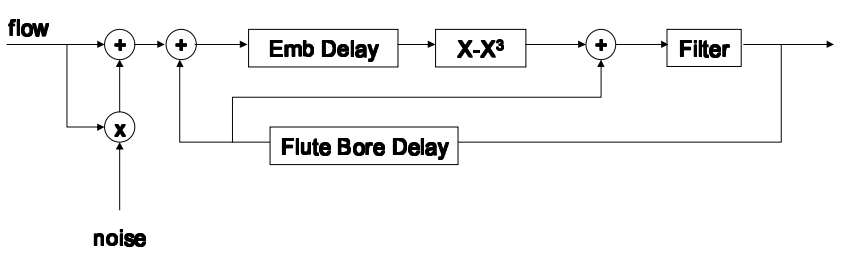
\includegraphics[width=14cm]{grafiki/flute_waveguide_mod}
	\captionsetup{justification=centering}
	\caption{Model falowodowy prostego instrumentu dętego drewnianego \cite{flute_prezka}.}
	\label{rys:flute_cook}
\end{figure}

%https://courses.cs.washington.edu/courses/cse467/05wi/pdfs/lectures/15-waveguideInstruments.pdf
Wejściem systemu przedstawionego na rysunku \ref{rys:flute_cook} jest przepływ powietrza (\emph{flow}), reprezentowany przez falę sinusoidalną. Szum (\emph{noise}) zostaje dodany w celu zasymulowania odgłosu wydechu flecisty. 
Interakcja między ustnikiem a komorą dźwiękową fletu przedstawiona została równaniem matematycznym $x-x^3$. Końcówka komory dźwiękowej odbija niskie częstotliwości - ta część została zasymulowana poprzez dodanie filtra dolnoprzepustowego przed wyjściem sygnału. Elementy \emph{Emb Delay} oraz \emph{Flute Bore Delay} to linie opóźniające, odpowiadające opóźnieniom fali w ustniku oraz w komorze dźwiękowej fletu. 
Obliczenie jednej próbki syntezowanego dźwieku, na podstawie rysunku \ref{rys:flute_cook}, wymaga 9 mnożeń oraz 6 operacji sumowania.

\subsubsection{Implementacja}
Implementację syntezy falowodowej w autorskim programie realizowanym na procesorze DSP,  wzorowano na schemacie \ref{rys:flute_cook}. Przepływ powietrza (\emph{flow}) został zaimplementowany jako fala sinusoidalna o odpowiedniej obwiedni \cite{flute_prezka}. Szum dochodzący do utworzonego sygnału został zasymulowany funkcją rand(), a jego amplituda została odpowiednio przeskalowana. Sygnały sinusoidy i szumu są sumowane, a następnie trafiają do pętli zamkniętej, którą zaimplementowano w postaci pętli "for". Charakter brzmienia takiego modelu fletu zmienia się w zależności od parametrów wzmocnienia obu linii sprzężenia zwrotnego oraz wartości opóźnień \emph{Emb Delay} i \emph{Flute Bore Delay}.

Jeden blok danych na procesorze DSP zawiera 1024 próbek. Linie opóźniające przesuwają próbki o kilkadziesiąt indeksów w tył. Oznacza to, iż pierwsza próbka nowego bloku danych, musi sięgnąć do poprzednio wygenerowanej tablicy. Do implementacji wykorzystano mechanizm tablicowy typu "ping-pong". Po wygenerowaniu pełnego bloku danych, pierwsza tablica przepisuje wszystkie wartości do drugiej. Następnie pierwsza tablica zostaje wyzerowana. Opóźnione próbki, do których należy się odnieść przy generowaniu nowego bloku danych, znajdują się w~drugiej tablicy. Takim mechanizmem zapewniono ciągłość generowanego sygnału, bez błędów obliczeniowych.

\subsection{Synteza na podstawie modelu ARMA}
W tym punkcie przedstawiono identyfikację modelu matematycznego fletu, na podstawie którego przeprowadzono później syntezę dźwięku. Do rozpoznania modelu instrumentu użyto tonu "A" razkreślnego o częstotliwości 440 Hz. Dźwięk wygenerowany w trakcie gry na flecie zmienia swoją charakterystykę w czasie. Oznacza to, iż jego model również zmienia się w trakcie granego przebiegu sygnału. Do identyfikacji wybrano te część nagrania, w której model instrumentu jest w~stanie ustalonym.

\subsubsection{Identyfikacja modelu}
Identyfikacja modelu matematycznego instrumentu została przeprowadzona poprzez manualne dopasowanie zer i biegunów modelu do widma nagrania.
Proces identyfikacji przeprowadzono w środowisku symulacyjnym Matlab. Na nagranym fragmencie sygnału przeprowadzono dyskretną transformację Fouriera za pomocą algorytmu FFT.

Identyfikacja procesu modelem wysokiego rzędu za pomocą funkcji wbudowanych w środowisku Matlab dawała lepsze rezultaty niż manualne szukanie pików i dolin. Taki sposób nie pozwalał jednak na późniejszą parametryzację modelu dla różnej wysokości dźwięków. Z tego powodu, autorzy zrezygnowali z automatycznej identyfikacji modelu ARMA.

% WYKRESSSSS
\begin{figure}[H]
	\centering
	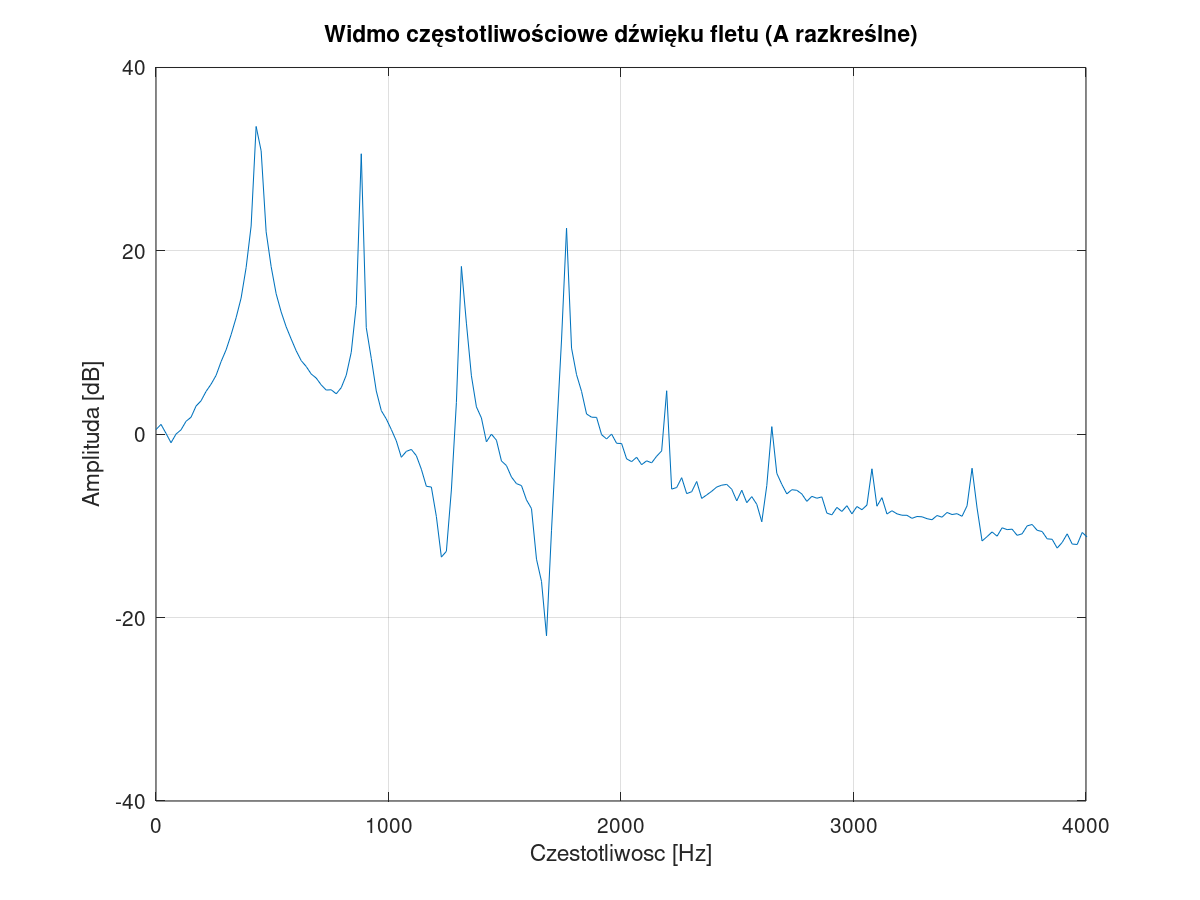
\includegraphics[width=12cm]{grafiki/flute_spectrum_orig}
	\captionsetup{justification=centering}
	\caption{Charakterystyka amplitudowa nagranego sygnału fletu.}
	\label{rys:flute_spectrum}
\end{figure}
% WYKRESSSS

Na rysunku \ref{rys:flute_spectrum} można zauważyć wyraźne piki oraz doliny charakterystyki częstotliwościowej nagranego sygnału. Siedem pierwszych pików charakterystyki zostało zinterpretowanych jako bieguny modelu, natomiast sześć pierwszych dolin zostało potraktowanych jako jego zera. Liczba wybranych pików i dolin, wziętych pod uwagę przy tworzeniu modelu, została dobrana na podstawie wzrokowej oceny ilości składowych harmonicznych, mogących mieć znaczny wpływ na ukształtowanie brzmienia zsyntezowanego instrumentu. Częstotliwości rezonansowe przetworzono według zależności:
\begin{equation} \label{equ:flute_bieguny}
p = 1-\frac{0.05}{A_{p}}e^{jf_{p}2\pi/F_{s}}
\end{equation}
\begin{equation} \label{equ:flute_doliny}
q = 1-\frac{0.05}{A_{q}}e^{jf_{q}2\pi/F_{s}}
\end{equation}
\begin{tabular}{ l l l l}
	gdzie: & $p$ &  - & bieguny modelu, \\
	&	$q$ & - &  zera modelu, \\
	&	$F_{s}$ & - &  częstotliwość próbkowania nagranego dźwięku,\\
	&	$f_{p,q}$ & - &  częstotliwość rezonansowa biegunów i zer modelu, \\
	&	$A_{p,q}$ & - &  amplituda rezonansu zer i biegunów. \\
\end{tabular} \\

Każdy pik charakterystyki został przetworzony na dwa bieguny odbite lustrzanie względem osi rzeczywistej na płaszczyźnie Z, według wzoru (\ref{equ:flute_bieguny}). Każda z dolin została odwzorowana jako dwa zera odbite lustrzanie względem osi Z, według zależności (\ref{equ:flute_doliny}).

Model ARMA zsyntezowanego fletu utworzono na podstawie wyznaczonych zer i biegunów. W~celu wygenerowania dźwięku z modelu w środowisku symulacyjnym, pobudzono go szumem białym. Następnie znormalizowano otrzymany sygnał, aby uniknąć przesterowań. Dźwięk wygenerowany z modelu przypominał brzmienie instrumentu z rodziny instrumentów dętych drewnianych. Wysokość wygenerowanego dźwięku odpowiadała tej z oryginalnego nagrania (440 Hz).

\subsubsection{Parametryzacja zidentyfikowanego modelu}
Model powinien mieć możliwość generowania dźwięków o różnej wysokości. Model zidentyfikowany metodą z poprzedniego punktu ma charakter statyczny - po pobudzeniu go szumem, zostaje wygenerowany z niego dźwięk zawsze o tej samej częstotliwości podstawowej (ton "A" razkreślny, na podstawie którego, model był identyfikowany). W celu osiągnięcia innego tonu na podstawie utworzonego modelu, należało dokonać jego parametryzacji. Polegała ona utworzeniu zależności między każdym biegunem i zerem modelu a pożądanym tonem, w oparciu o zasady przyjęte w protokole MIDI.

\begin{equation} \label{equ:flute_param}
\openup\jot
\begin{aligned}[t]
f_{p} = f_{A^{1}}(\sqrt[12]{2})^{n-k} \\ 
\end{aligned}
\qquad\qquad % adjust to suit
\begin{aligned}[t]
k = 69, 57, 50, 45, 42, 38 \\
\end{aligned}
\end{equation}
\begin{tabular}{ l l l l}
	gdzie: & $f_{p}$ &  - & częstotliwość rezonansowa biegunu modelu, \\
	&	$f_{A^{1}}$ & - &  częstotliwość dźwięku A razkreślnego (440 Hz), \\
	&	$n$ & - &  numer aktualnie wybranego klawisza w systemie MIDI.\\
\end{tabular} \\

Na podstawie wzoru (\ref{equ:wpr_dzwiek}), została utworzona zależność biegunu od częstotliwości podstawowej zidentyfikowanego modelu. Przedstawiono ją we wzorze (\ref{equ:flute_param}). Podobny mechanizm zastosowano dla zer modelu. 

\begin{figure}[H]
	\centering
	\includegraphics[width=11.5cm]{grafiki/Model_B_A}
	\label{rys:por_mod_flet}
	\captionsetup{justification=centering}
	\caption{Porównanie widma modeli ARMA fletu dla dzwieku "B" razkreślnego (wykres przesuniety w~prawo) i "A" razkreślnego (wykres przesunięty w lewo).}
	\label{rys:por_mod_flet}
\end{figure}
Można zauważyć na rysunku \ref{rys:por_mod_flet}, że dla różnych tonów wszystkie piki oraz doliny opisane zidentyfikowanym modelem przesuwają się w dziedzinie częstotliwości. Oznacza to, iż pobudzony model może wygenerować dźwięk o różnej wysokości, w zależności od parametru $n$ występującego we wzorze (\ref{equ:flute_param}).


\subsubsection{Implementacja}
W autorskim programie dla procesora DSP, syntezę dźwięku za pomocą zidentyfikowanego modelu ARMA, zaimplementowano jako przetwarzanie szumu poprzez filtr IIR. Współczynniki filtru uzyskano z przeprowadzonej wcześniej symulacji w środowisku Matlab. 
% O tym jak precyzja zmieniala wyniki!! Na floatach nie dziala.
W celu zmniejszenia złożoności obliczeniowej, do obliczania próbek zastosowano typ zmiennych o pojedynczej precyzji (float). Spowodowało to sytuację, w której wartości generowanego dźwięku fletu narastały do nieskończoności. Działo się to na skutek zbyt niskiej precyzji powodującej błędy numeryczne w~filtrze ze sprzężeniem zwrotnym. Po modyfikacji typu zmiennych na zmienne o podwójnej precyzji (double), uzyskano pożądane rezultaty - stabilny model ARMA i sygnał wyjściowy odpowiadający dźwiękowi instrumentu dętego drewnianego.

% opisac jak zaimplementowano filtr IIR ?? - tak
% przedstawic splot sygnału

Algorytm przesyłania kolejnych bloków danych z próbkami dźwięku do przetwornika DAC jest taki sam, jak opisany w podrozdziale \ref{sec:fm_gen_przeb}. Z uwagi na dużą złożoność obliczeniową, w syntezie fletu z wykorzystaniem modelu ARMA nie zaimplementowano mechanizmu polifonii.
Interfejs użytkownika dla syntezy dźwięku fletu ogranicza się do włączenia tej opcji za pomocą przycisku "Enable". Nie ma możliwości zmiany parametrów syntezy przez użytkownika. Jest to spodowodowane bardzo dużą wrażliwością modelu na nawet najmniejsze zmiany parametrów.

\subsection{Wyniki}
Poniżej przedstawiono wyniki syntezy dźwięku fletu dla obydwu metod - falowodowej oraz z~wykorzystaniem modelu ARMA.

\begin{figure}[H]
	\centering
	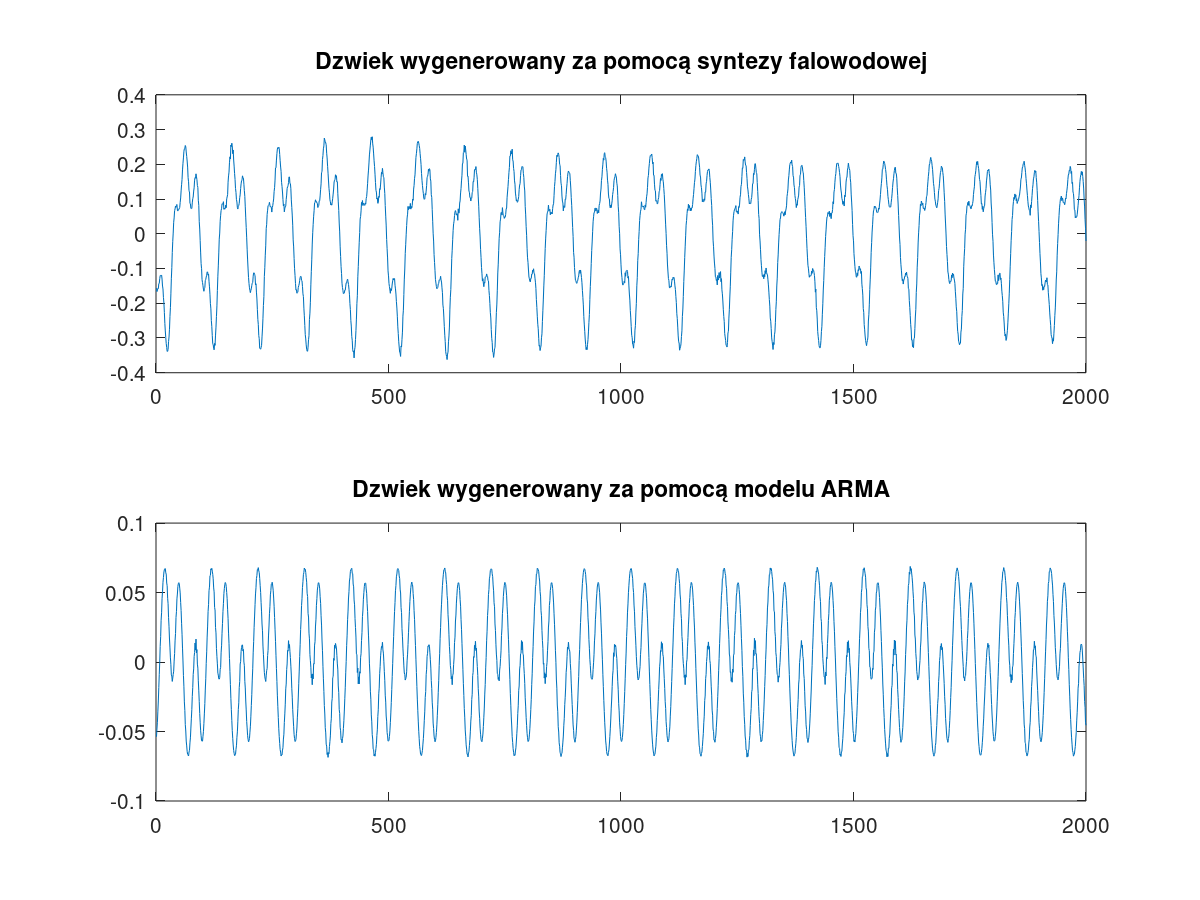
\includegraphics[width=12cm]{grafiki/flute_porownanie_syntez_symulacja}
	\captionsetup{justification=centering}
	\caption{Porównanie symulacji dzwieku fletu dla syntezy falowodowej i syntezy za pomocą modelu ARMA fletu.}
	\label{rys:por_synt_flet}
\end{figure}

% TO pierwsze zdanie po obserwacji periodogramow
Można zauważyć, iż porównanie syntezy instrumentu dętego, które zostało przedstawione na rysunku \ref{rys:por_synt_flet}, dało zupełnie różne wyniki dla obu metod. Po odpowiednim doborze parametrów modelu falowodowego, takich jak wzmocnienie sprzężenia pętli zamkniętej oraz wartość opóźnienia, uzyskane brzmienie jest bardziej zbliżone do barwy fletu. Jego barwa zmienia się w czasie. W celu otrzymania lepszych wyników syntezy za pomocą modelu ARMA, należałoby prawdopodobnie użyć modelu zmiennego w czasie (kilku modeli). Dodatkowo, aby generowany dźwięk był bardziej zbliżony do naturalnego, zidentyfikowany model powinien być wyższego rzędu. Miałoby to jednak negatywny wpływ na wykonywanie pracy programu dla DSP w czasie rzeczywistym.

% Można dodać periodogram uśredniony 